\graphicspath{ {./images/} }
\begin{problem}%
{Ход конём-2}%
{\textsl{стандартный ввод}}%
{\textsl{стандартный вывод}}%
{1 секунда}%
{256 мегабайт}{}

Дана прямоугольная доска $N \times M$ ($N$ строк и $M$ столбцов). В левом верхнем углу находится шахматный конь, которого необходимо переместить в правый нижний угол доски. При этом конь может ходить только так, как показано на рисунке:

\begin{center}
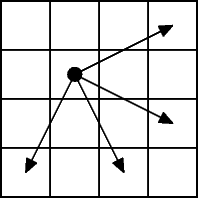
\includegraphics{2962.png}
\end{center}

Необходимо определить, сколько существует различных маршрутов, ведущих из левого верхнего в правый нижний угол.

\InputFile

В первой строке входного файла находятся два натуральных числа N и M ($1 \le N, M \le 15$).  

\OutputFile

В выходной файл выведите единственное число количество способов добраться конём до правого нижнего угла доски.

\Examples

\begin{example}
\exmp{
4 4
}{%
2
}%
\exmp{
7 15
}{%
13309
}%
\end{example}
\end{problem}
